\documentclass[11]{article}
\usepackage[utf8]{inputenc}

\usepackage{cite}
\usepackage{multicol}
\usepackage{float}
\usepackage{graphicx}
\usepackage[margin=1.25in]{geometry}
\usepackage{subcaption}
\author{Xavier Martín Ballesteros and Adrià Cabeza Sant'Anna \\ \small UNIVERSITAT POLITÈCNICA DE CATALUNYA}
\title{Flower detection using features\\ \large{Computer Vision, UPC}}
\date{\today}

\begin{document}
\maketitle
\vspace*{\fill}
\begin{center}

\includegraphics[scale=0.4]{UPClogo.png}\par\vspace{1cm}
\end{center}
\newpage
\tableofcontents
\newpage 

\section{Introduction}
The aim of this assignment is to classify 12 different types of flowers using feature extraction. The different flower types are the following:
\begin{multicols}{3}
\begin{itemize}
\item BotodOr 
\item Crocus  
\item Fadrins   
\item Gerbera 
\item Hemerocallis 
\item Narcis
\item Buixol
\item DentdeLleo 
\item Fritillaria  
\item Girasol 
\item Lliri     
\item Viola

\end{itemize}
\end{multicols}

We have first implemented several ways to extract features that we believed could be key in order to classify correctly the flowers, we tested them, and using different classifiers (decisions trees, SVM or random forest) have tested the accuracy, specificity or sensitivity. 

\section{Descriptors}
\label{sec:desc}
In the following sections we will introduce different descriptors we have used to find those valuable features.

\subsection{Compactness}
One of the first descriptors we came up with when observing the different species of flowers was the \textbf{compactness}, that is the ratio of the perimeter to the area of the region. Since the shape and the size of each flower really varies, we think it can be a good discriminator. 

The measure takes a minimum value of 1 for a circle. However, objects which have an elliptical shape or a
boundary that is irregular rather than smooth, will
decrease the measure. On the other hand, objects that have complicated, irregular boundaries will have larger compactness.

\medskip

To implement it we do need two things: \textbf{perimeter}(\textit{P}) and \textbf{area}(\textit{A}).

$$C= \frac{(P^2 / Area)} {4*\pi}$$
  \medskip
  
 To get the area we have used Matlab's \textbf{regionprops} utility, and to get the perimeter we have made \textbf{an erosion and a substraction with the original image}. Then, we have counted the number of pixels in white. 
 \medskip 
 
 \noindent In this example, we compare a \textit{Hemerocallis} and a \textit{Botó d'Or} flowers. As the \textit{Botó d'Or} image is more similar to a circle than the \textit{Hemerocallis} one, we should have smaller values for it.
 
 \begin{figure}[H]
    \begin{subfigure}[t]{.49\linewidth}
    \centering
  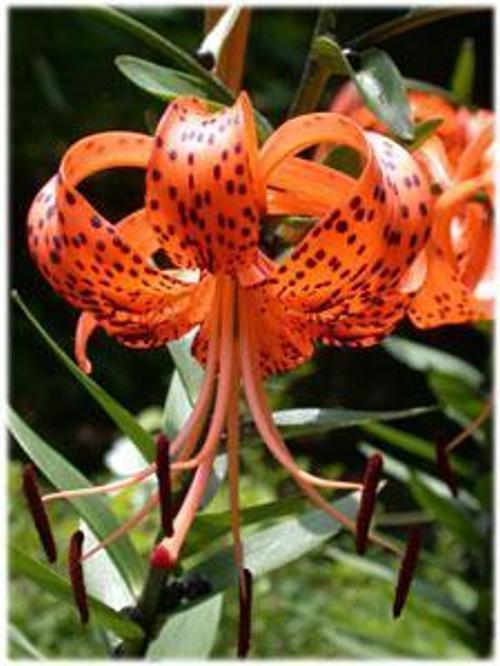
\includegraphics[scale=0.23]{images/compactness1.jpg}
  \caption{Compactness: \textbf{28.10}}
  \label{original}
    \end{subfigure}
    \begin{subfigure}[t]{.49\linewidth}
    \centering
    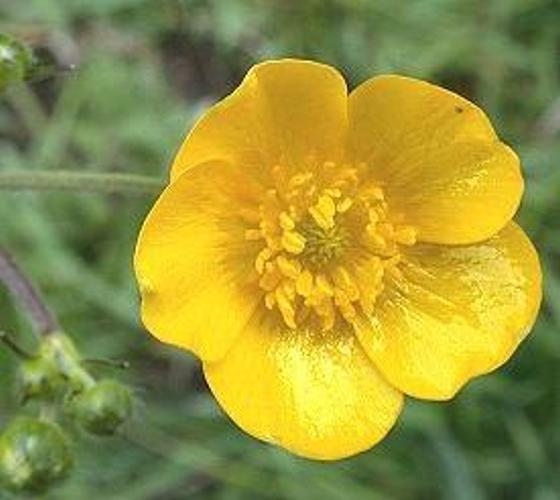
\includegraphics[scale=0.28]{images/compactness2.jpg}
    \caption{Compactness: \textbf{0.78}}
    \label{skez}
    \end{subfigure}
    \caption{Comparison of compactness}
\end{figure}

\subsection{Color}
Even though there are some types of flowers that can have different colors, most of them show always the same one or two colors. Thus, the color is really important in order to distinguish one specie from another. To do it we have used  the Mathworks utiliy: \textbf{image2palette\cite{image2palette} which uses k-means color clustering}. We executed the k-means with 4 clusters (one is for the black, which is always present) to get the most important colors.

Moreover, we have also the percentage of pixels that belong to each cluster. Consequently, we will not only use the cluster colors as a feature but also its percentages. We have to remark that before adding the percentage feature to the feature vector, we delete the black percentage and then normalize the other three values.

\medskip

This is an example with a \textit{Viola} picture:
 
\begin{figure}[H]
	\centering
	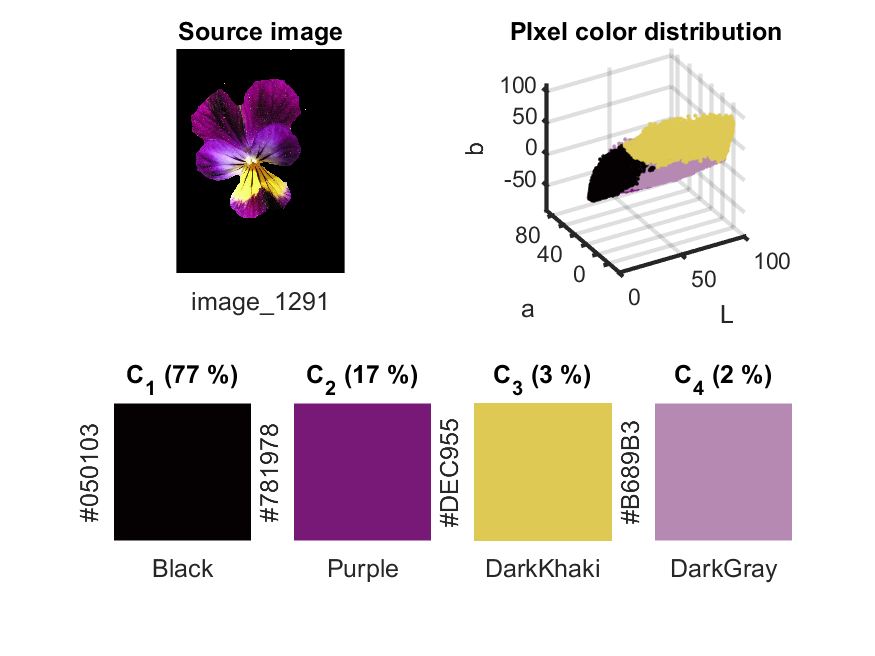
\includegraphics[scale=0.85]{images/colorOriginal.png}
	\caption{Example of our color feature extraction}
	\label{color}
\end{figure}

\subsection{Number of petals}

This descriptor was one of the most difficult to think of. It can be done in several ways so we first had to choose in which way we wanted to attack the problem. In our case we decided to \textbf{skeletonize the flower}.
\medskip

To do so we used \textbf{bwmorph(image, 'skel', inf)} from Matlab. This	 creates the skeleton iterating as many times as necessary in order to not see any change between iterations (until it converges). Then we observed that sometimes the skeleton did not touch the contourn of the flower so we could not really count the petals. To solve it, we applied an small erosion using a disk of radius 4 as the structural element. The value of the disk structure was chosen based on several trials.

Finally, we use \textbf{bwlabel(image, X-connected)} to label the image in order to obtain the number of petals. In our case, we have computed it using a value of 4 as the connectivity.

\medskip

\noindent In this example using \textit{Boto d'Or} we get as a result 5 petals:
\begin{figure}[H]
    \begin{subfigure}[t]{.49\linewidth}
    \centering
  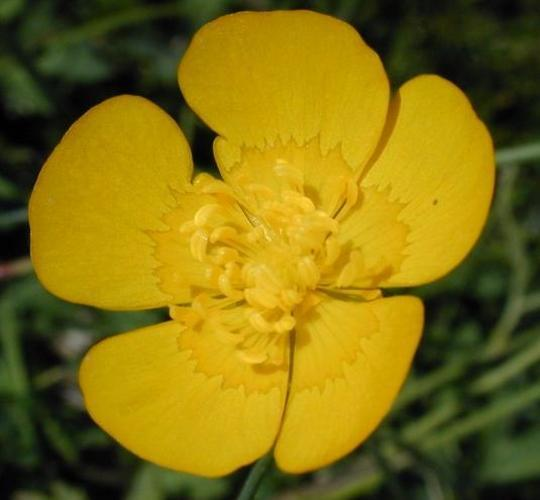
\includegraphics[scale=0.25]{images/numberOfPetalsOriginal.jpg}
  \caption{Original}
  \label{original}
    \end{subfigure}
    \begin{subfigure}[t]{.49\linewidth}
    \centering
    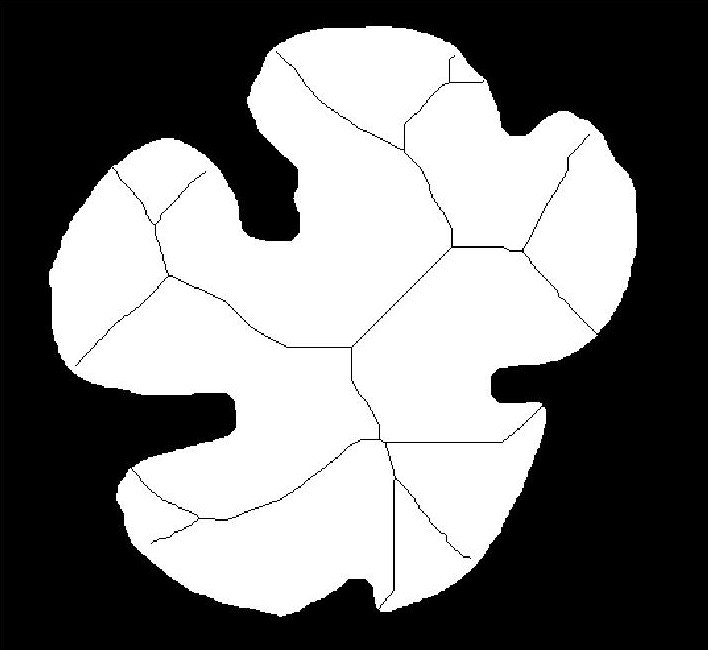
\includegraphics[scale=0.2]{images/numberOfPetals.jpg}
    \caption{Skez of the image}
    \label{skez}
    \end{subfigure}
\end{figure}

\subsection{Relative position of the centroid}

Just evaluating the position of the centroid would have been useless, it is not a feature of the flower per se. It can vary depending on the angle of the photo or the distance. However, if we calculate the relative position with respect to the flower's bounding box, we can get really powerful information. 
\\

This two flowers, for example, should have really different values for this descriptor and it could be key in order to differenciate them in our classifier:
\begin{figure}[H]
    \begin{subfigure}[t]{0.45\textwidth}
    \centering
  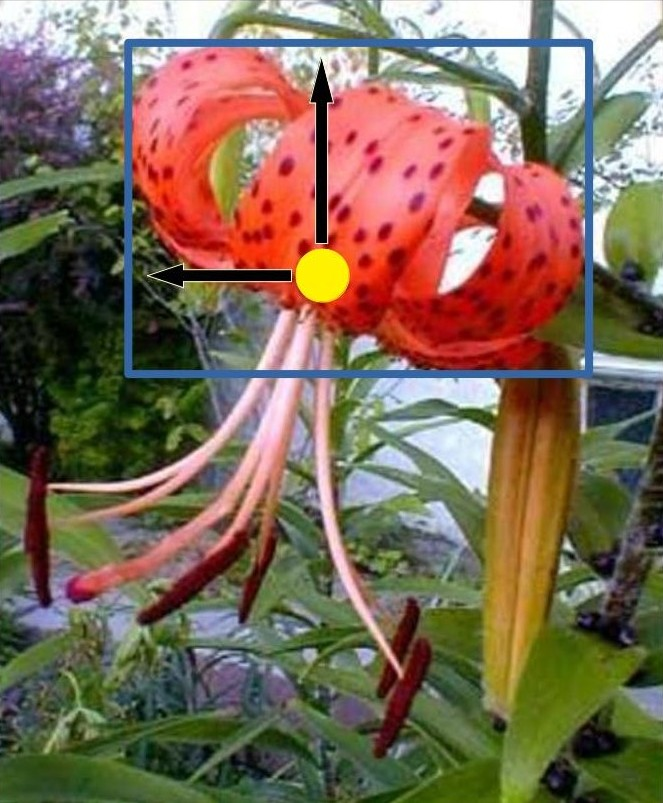
\includegraphics[scale=0.2]{images/hemerocallisCentroid.jpg}
    \caption{Centroid and bounding box of a \textit{Hemerocallis}}
    \label{centroidHemerocallis}
    \end{subfigure}
    \begin{subfigure}[t]{0.45\textwidth}
    \centering
    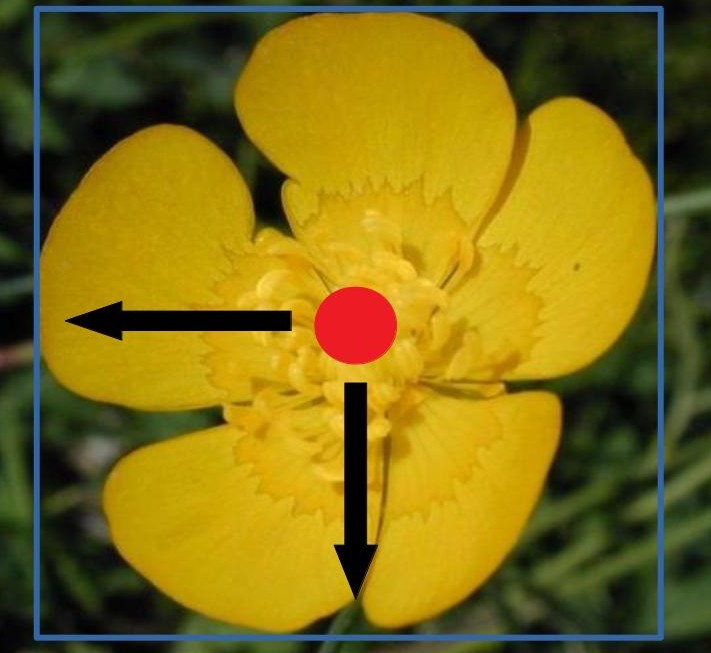
\includegraphics[scale=0.2]{images/GirasolCentroid.jpg}
    \caption{Centroid and bounding box of a \textit{Girasol}}
    \label{centroidgirasol}
    \end{subfigure}
\end{figure}

The way our descriptor is implemented is the following: we get the first and last pixels of X and Y axis in order to create the \textbf{bounding box}, then using \textbf{regions props} we get the \textbf{centroid of the flower} and finally we calculate the \textbf{relative position} of the centroid over the bounding box. 
\medskip

\begin{figure}[H]
	\centering
	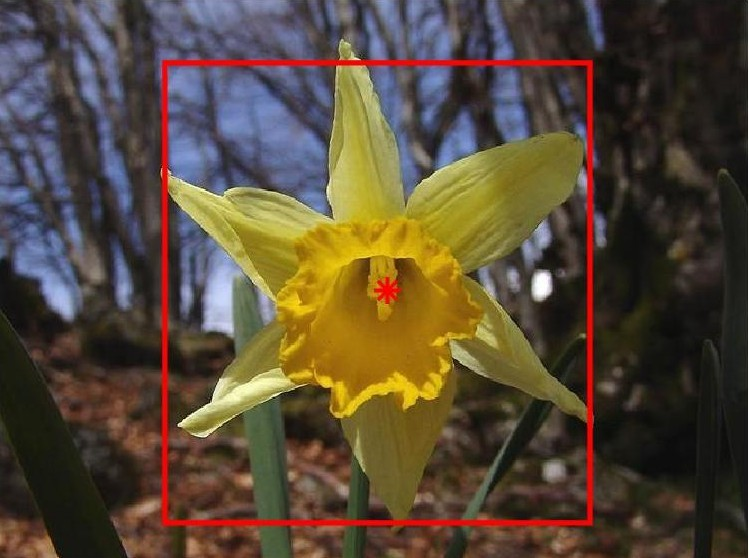
\includegraphics[scale=0.35]{images/centroid.jpg}
	\caption{Example of centroid and bounding box}
	\label{centroidNarcis}
\end{figure}


\subsection{Fourier descriptor: Shape}
It is known that we can use the Fourier transform to analyse and characterize the shape of a boundary. Since there are some flowers like the \textit{Hemerocallis} or the \textit{Girasol} that have a very specific shape, we believe that \textbf{the shape} can be a great descriptor.  We have only got the first and last \textbf{N} values of the vector as features, where \textbf{N} marks the level of detail we want of the shape.

\begin{figure}[H]
    \begin{subfigure}[t]{0.45\textwidth}
    \centering
  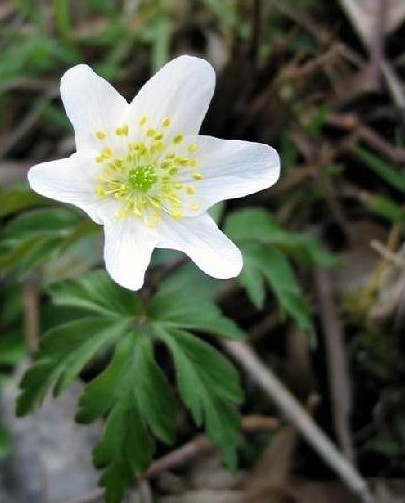
\includegraphics[scale=0.25]{images/originalfourier.jpg}
    \caption{Original}
    \label{originalfourier}
    \end{subfigure}
    \begin{subfigure}[t]{0.45\textwidth}
    \centering
    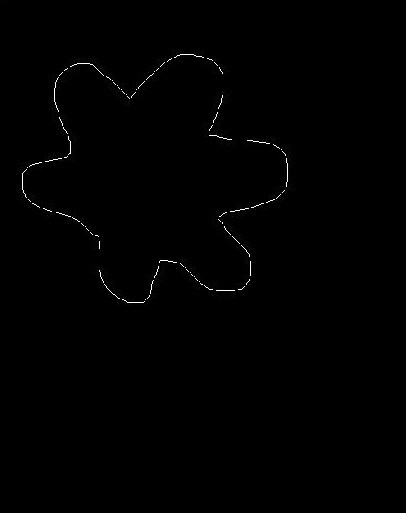
\includegraphics[scale=0.25]{images/shape.jpg}
    \caption{Shape}
    \label{fourier2}
    \end{subfigure}
    \label{fourier}
    \caption{Fourier descriptors}
\end{figure}


\subsection{Hogs form: Orientation}
Previously we have introduced a way to describe information about the shape. However, there are other ways to describe it. 
\\
As we wanted to have as proper features as possible, we have also implemented HOGs (histogram of oriented gradients), which basically describes \textbf{the shapes as the distribution of intensity gradient and edge directions}.

To do it, we have computed the first derivatives of \textit{x} and \textit{y} to obtain the gradient. Then, we have computed the histogram of the gradients using the number of bins specified in the input. In our case, we have used 16 bins.

\begin{figure}[H]
    \begin{subfigure}[t]{0.45\textwidth}
    \centering
  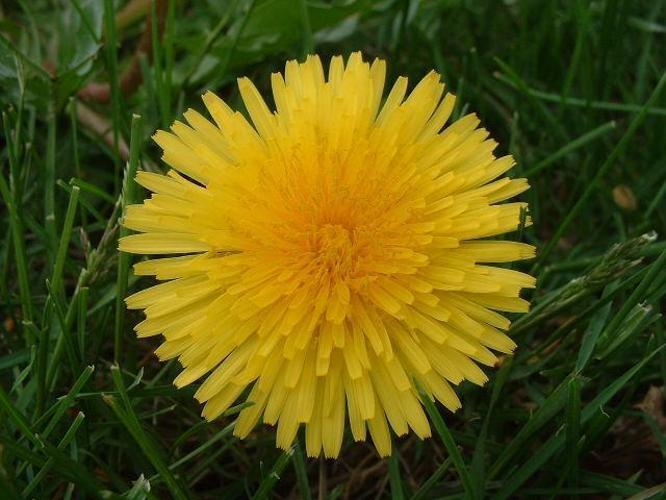
\includegraphics[scale=0.234]{images/originalhogg.jpg}
    \caption{Original}
    \label{originalhogg}
    \end{subfigure}
    \begin{subfigure}[t]{0.45\textwidth}
    \centering
    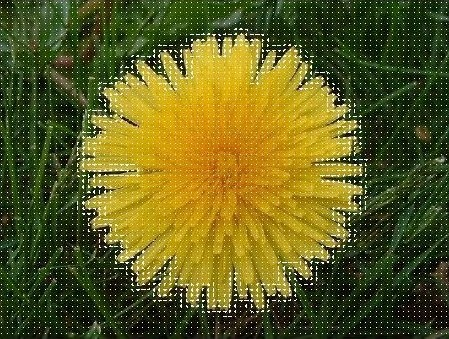
\includegraphics[scale=0.345]{images/hogg.jpg}
    \caption{Hog features}
    \label{hogg2}
    \end{subfigure}
    \label{hogg}
    \caption{HOG descriptors}
\end{figure}



\section{Classifiers}

Once we have obtained the feature matrix, where each column represent a feature and each row represent an image, we have used the \textbf{Classification Learner App} from Matlab to see the accuracy we get with different types of classifiers. For the classifiers, we have chosen the \textbf{Cross-Validation} method with 50 folds to examine the prefictive accuracy of the fitted models.

The Cross-Validation method gives a good estimate of the predictive accuracy of the final model trained with all the data. It is very recommended for small datasets, which is our case. It partitions the dataset into \textit{k} disjoint folds. For each of them it trains the model and finally it calculates the average test error over all folds.

We have used a Random Forest as our classifier. To obtain it, we have used \textbf{fitcensemble} with Method \textit{Bag}, which stands for "bootstrap aggregation", and Tree as Learner. It has as parameters the number of learners (trees) and the maximum number of splits per tree.

The results with this App can be found in Section \ref{sec:results}.

\section{Experiments}

\subsection{Feature variables}

The first thing we had to do was to obtain the characteristics that seem suitable for describing each type of flower (see Section \ref{sec:desc} to see what features we used). Nevertheless, all features (except the compactness and the bounding box) have some variables that need to be fitted.

In this first experiment we have focused on giving the best possible values to those variables. To do it, we have worked on each feature "isolated" from the rest so that the predictions could only vary because of the change of the feature we were working at. We have started by setting a random value two times to a variable and comparing the results. Afterwards, we set again another value (greater or lower depending on the results obtained) and compared the result with the best result of the previous two results. This has been done until the results have been very similar. Thus, the value for the variable has been the one that has given us the best result.

For example, in the number of petals we have been modifying the radius of the disk and observing the number of petals from the output. Depending on that value, we have increased/decreased the radius.
\\
\begin{center}
\centering
\begin{tabular}{ |c|c| } 
 \hline
 \textbf{Feature} & \textbf{Variable}  \\ 
   \hline
  \hline
 \textbf{Color} & nClusters = 4  \\ 
  \hline
 \textbf{Compactness} & -  \\ 
   \hline
 \textbf{Number of petals} & SE radius = 4  \\ 
   \hline
 \textbf{Fourier} & N = 6  \\ 
   \hline
 \textbf{HOG} & bins = 16  \\ 
   \hline
 \textbf{Bounding box} & Take contour = NO  \\ 
 \hline
\end{tabular}
\end{center}

\medskip

Even though we though that the contour would be crucial for the bounding box (especially for the \textit{Hemerocallis}) we have seen that we got worse results when using also the contour. We concluded that this happens due to the fact that some segmented images have contour in its borders. This means that there is contour in places where there is no flower.

\subsection{The dataset and experimental procedure for the classification}

We have used a dataset consisting of 681 images divided into 12 flower classes. Each class consists of between 46 and 75 images. The dataset is divided into a training set and a validation set. The training set consist of the 80\% of images per class (539 in total). The validation set consist of the remaining 20\% of images (142 in total). Figure \ref{fig:barplot} shows the distribution of the number of images over all the classes. 

\begin{figure}[H]
	\centering
	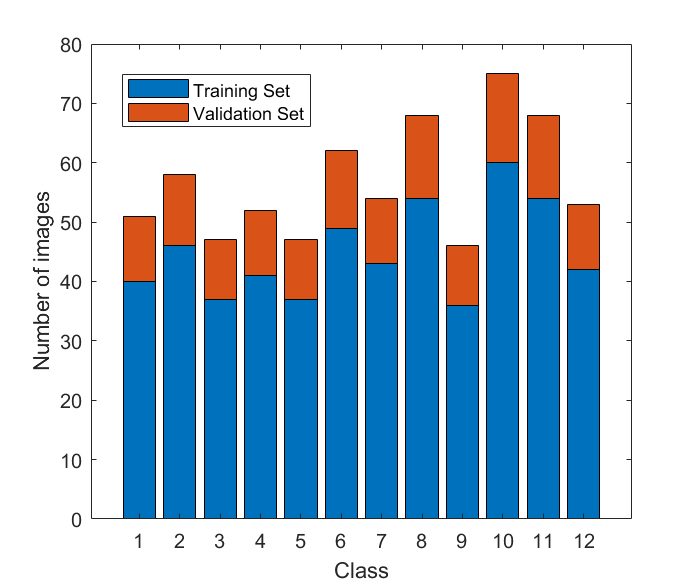
\includegraphics[scale=0.45]{./images/barplot}
	
	\caption{The distribution of the number of images over the 103
classes.}
	\label{fig:barplot}
\end{figure}

We have trained all the classifiers with the training set and we have selected the one with the best accuracy. Then, we have used it to classify the images from the validation set. We have computed the accuracy for each class. The final performance is the classification averaged over all classes (not over all images).

\subsection{Segmentation}

Some of the pictures that were given did not have a proper segmentation. Moreover, if we wanted to use different pictures from another sources, we needed a nice and automated way to segmented them since most of our descriptors use the segmentation.\\
\medskip

To do so we tried several methods because segmentation can be really difficult depending on the image. Some of the methods we tried were \textbf{Otsu}, \textbf{k-means with 3 or 4 clusters}, \textbf{superpixels and region growing} or \textbf{fast marching}. We also considered another type of algorithms called \textbf{graph-based segmentation} but they are not easy to automate so we discarted them. In the following examples, you can see some of the bad segmentations those methods gave us:

\begin{figure}[H]
    \begin{subfigure}[t]{0.45\textwidth}
    \centering
  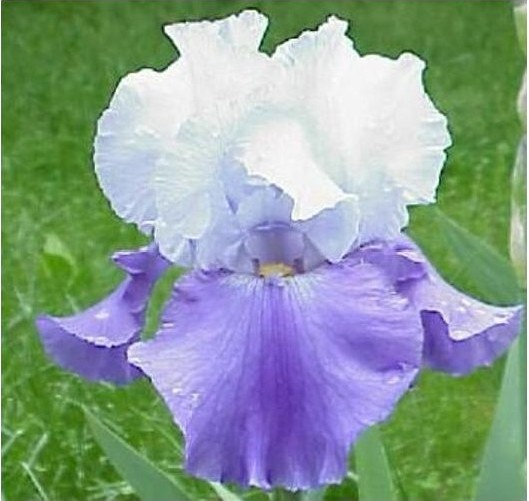
\includegraphics[scale=0.13]{images/segmentation0.jpg}
    \caption{Segmentation using Otsu}
    \label{segmentation0}
    \end{subfigure}
    \begin{subfigure}[t]{0.45\textwidth}
    \centering
    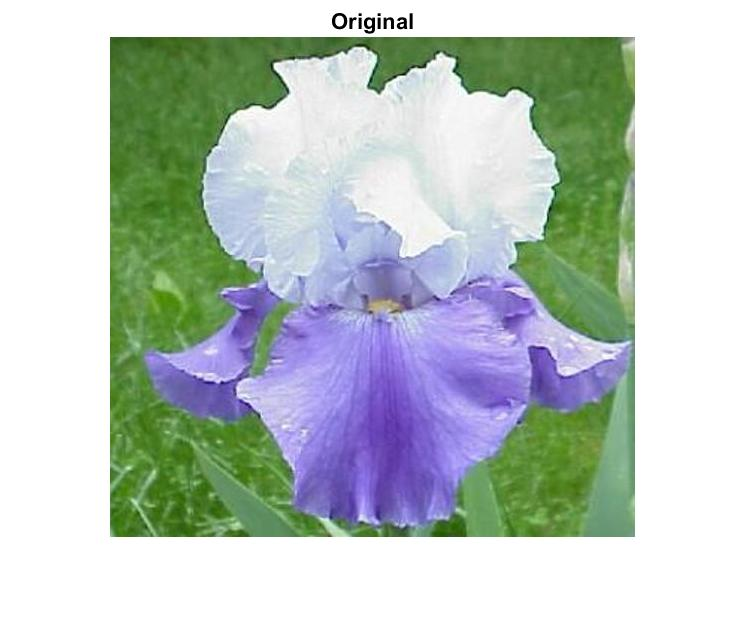
\includegraphics[scale=0.35]{images/segmentation1.jpg}
    \caption{Segmentation using k-means}
    \label{segmentation1}
    \end{subfigure}
\end{figure}

\begin{figure}[H]
    \begin{subfigure}[t]{0.45\textwidth}
    \centering
  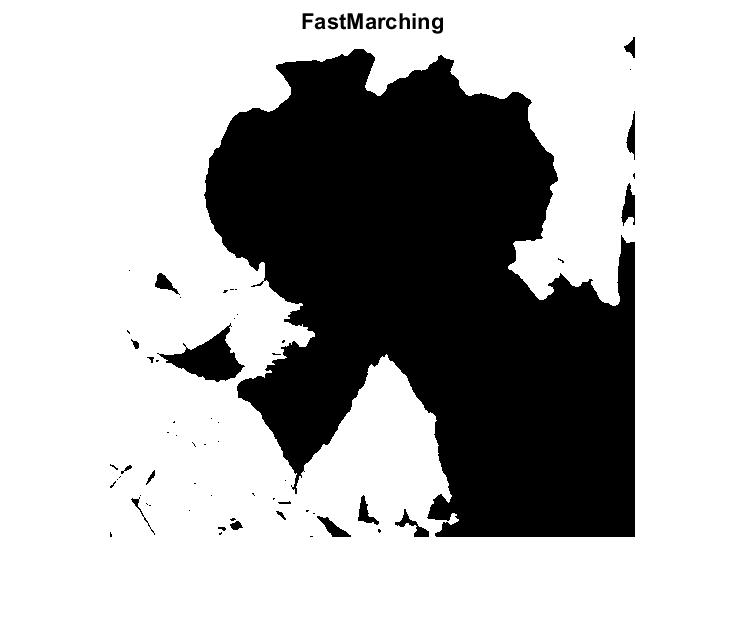
\includegraphics[scale=0.20]{images/segmentation2.jpg}
    \caption{Segmentation using }
    \label{Segmentation using }
    \end{subfigure}
    \begin{subfigure}[t]{0.45\textwidth}
    \centering
    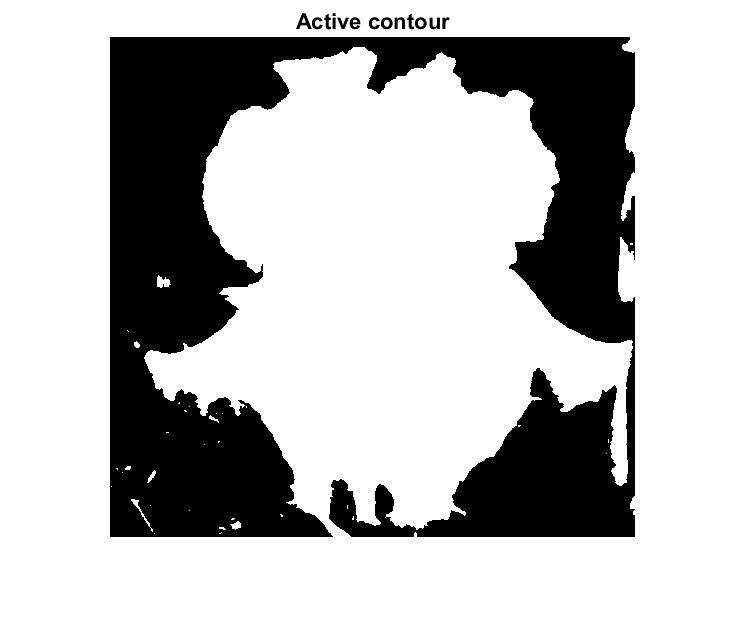
\includegraphics[scale=0.20]{images/segmentation3.jpg}
    \caption{Segmentation using }
    \label{segmentation3}
    \end{subfigure}
    \label{segmentationALL}
    \caption{Examples of bad segmentations with different methods}
\end{figure}

Finally, we did realize that it was nearly impossible to get a perfect segmentation method, it really depends on the image; so we decided to use the \textbf{active contour} method which seems to get us the bests results. This method segments an image into foreground and background using the active contour algorithm, also called \textit{snakes}. During an interative process, those \textit{snakes} move to find object boundaries.

\begin{figure}[H]
    \begin{subfigure}[t]{0.45\textwidth}
    \centering
  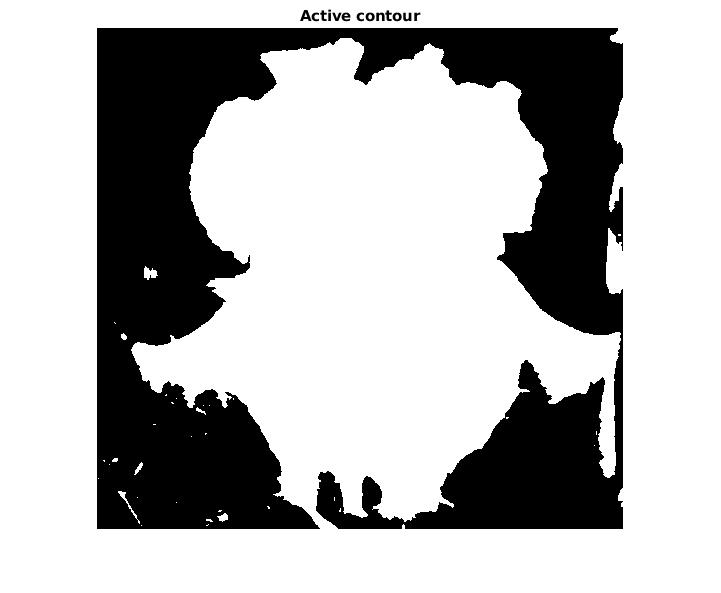
\includegraphics[scale=0.20]{images/segmentation4.jpg}
    \end{subfigure}
    \begin{subfigure}[t]{0.45\textwidth}
    \centering
    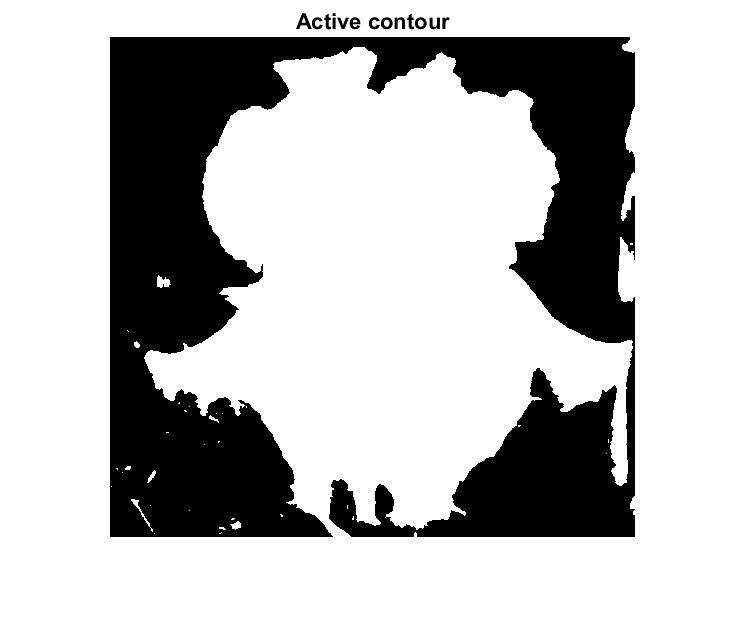
\includegraphics[scale=0.20]{images/segmentation3.jpg}
    \end{subfigure}
    \label{segmentation4}
    \caption{Examples of segmentations with active contour method}
\end{figure}


\section{The \textit{zero} class}

In order to increase the precision of our model, we have added a new class called \textit{zero}. This class represents all the flowers that are not from any of the 12 species that we are observing.
\medskip

To implement it we have written a script that \textbf{crawls google images and downloads photos of other species of flowers}. This will be very useful to create our dataset of \textit{zero} flowers. Morover, since these images are not segmented, we have looked for another source of flower pictures. In this case we have used \textbf{the Flowers Dataset from the Visual Geometry Group} (University of Oxford)\cite{Flower dataset}. This approach will help us to save time because we will have some flowers segmented by us (reviewed manually afterwards) and some already segmented (which we suppose are already correct).
\medskip

Our approach will consists in not training our classifier with that photos: we will assign a picture to that class if the confidence is less than a threshold. To test if actually works we will use the already mentioned test. 

Some of the flowers that can be seen in our \textit{zero} flower dataset are:
\begin{figure}[H]
    \begin{subfigure}[t]{0.45\textwidth}
    \centering
  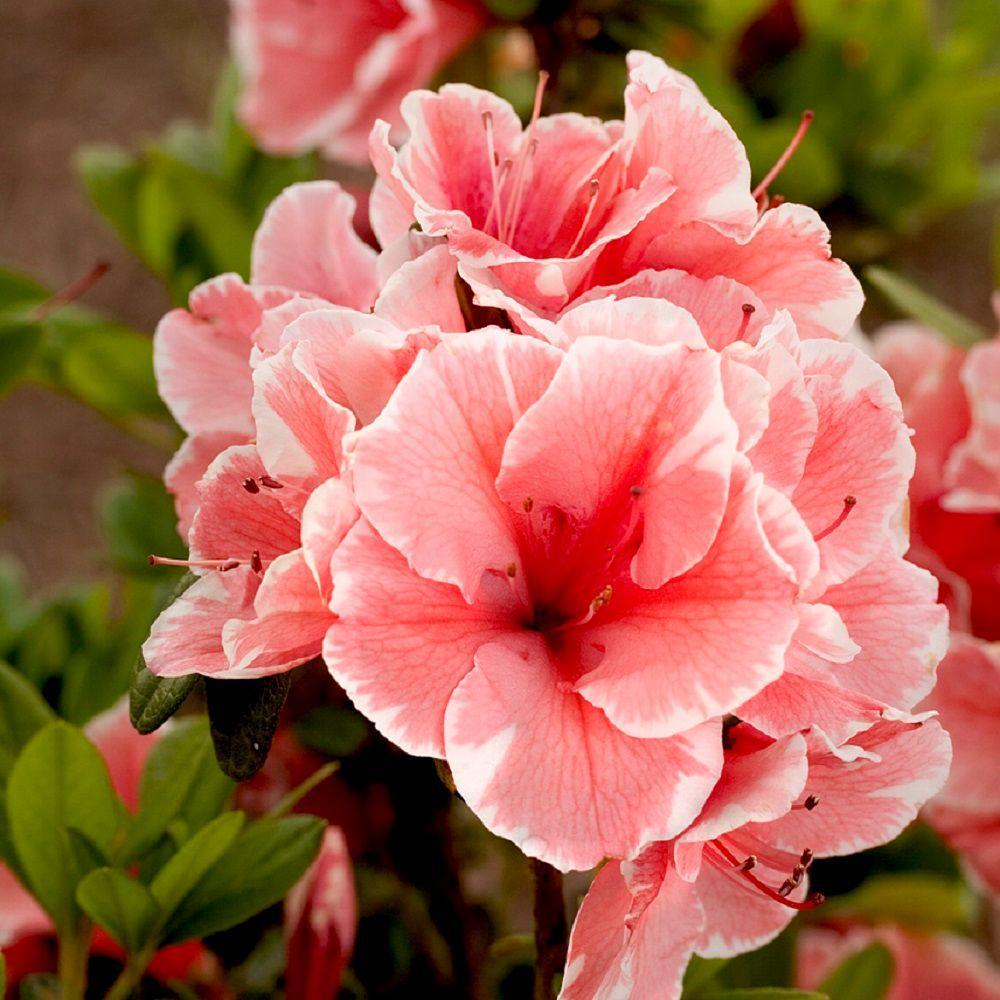
\includegraphics[scale=0.13]{images/azalea.jpg}
    \caption{Azalea}
    \label{azalea}
    \end{subfigure}
    \begin{subfigure}[t]{0.45\textwidth}
    \centering
    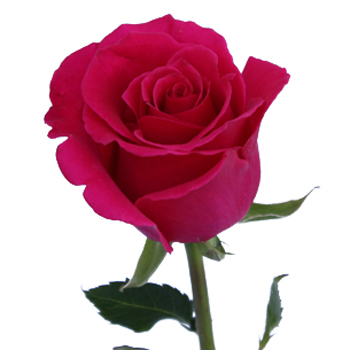
\includegraphics[scale=0.35]{images/roses.jpg}
    \caption{Roses}
    \label{roses}
    \end{subfigure}
\end{figure}

\begin{figure}[H]
    \begin{subfigure}[t]{0.45\textwidth}
    \centering
  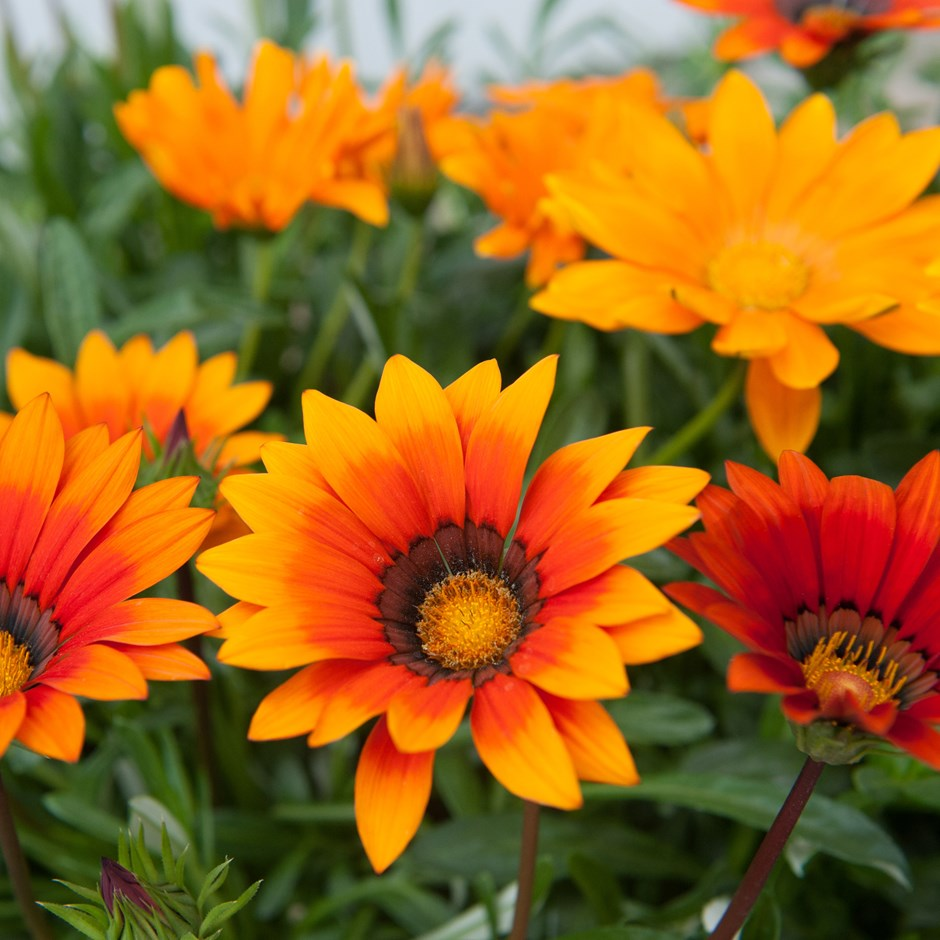
\includegraphics[scale=0.20]{images/gazania.jpg}
    \caption{Gazania}
    \label{gazania}
    \end{subfigure}
    \begin{subfigure}[t]{0.45\textwidth}
    \centering
    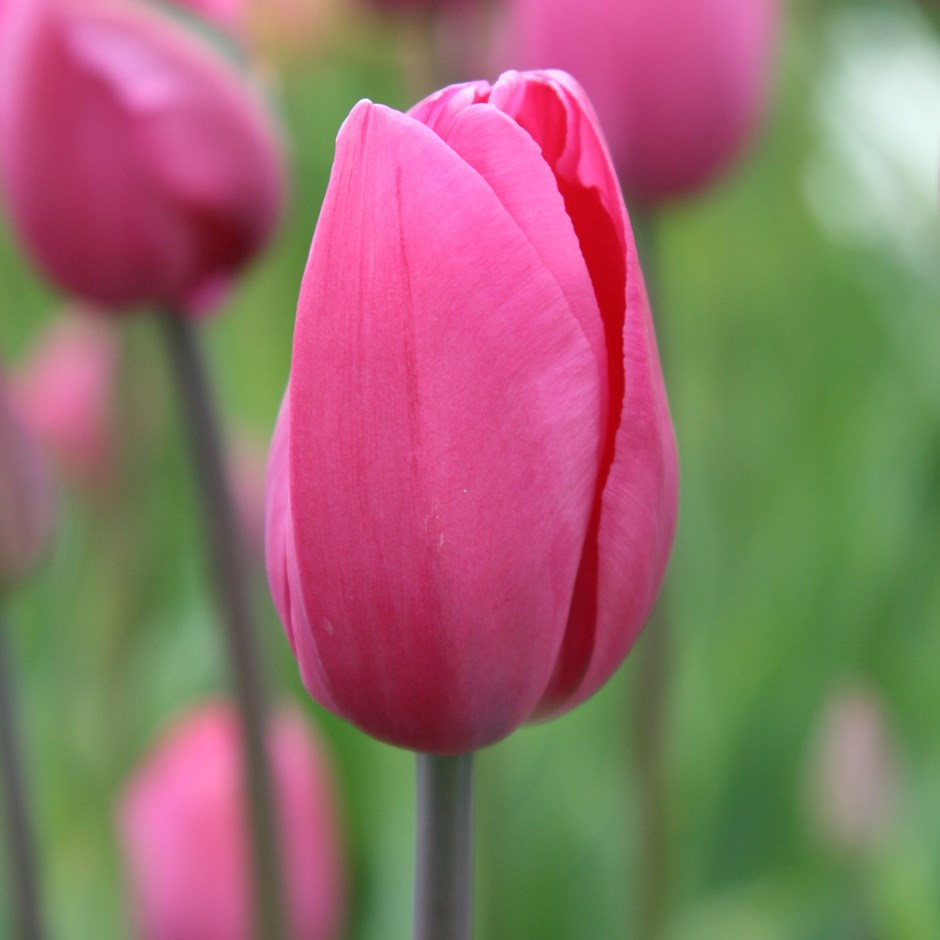
\includegraphics[scale=0.20]{images/tulip.jpg}
    \caption{Tulip}
    \label{tulip}
    \end{subfigure}
    \label{zero}
    \caption{Zero class flowers}
\end{figure}


\section{Data augmentation}
In order \textbf{to strenghten our descriptors} we have also used the following public repository:  \textit{Albumentation: fast image augmentation library and easy to use wrapper around other libraries} \cite{Albumentations}, which proporcionates facilities to augment the dataset including several transformations like: flipping, blurring, RGB Shifting, Random contrast, Random brightness, etc...
\medskip

To decide which transformations we wanted to apply, we looked first to our descriptors and the importance of each feature. For example, we discarted the Channel Shuffle because we believe that the color is very important for our implementation. Then, based on trial and error, we picked some of them which gave us an overall better result. Finally we are using random variations of:
\begin{itemize}
    \item Brightness and Contrast
    \item Blur
    \item Rotations
    \item Flips
\end{itemize}
For example let's suppose that we are working with this \textit{Boto d'Or} image:
\begin{figure}[H]
    \centering
    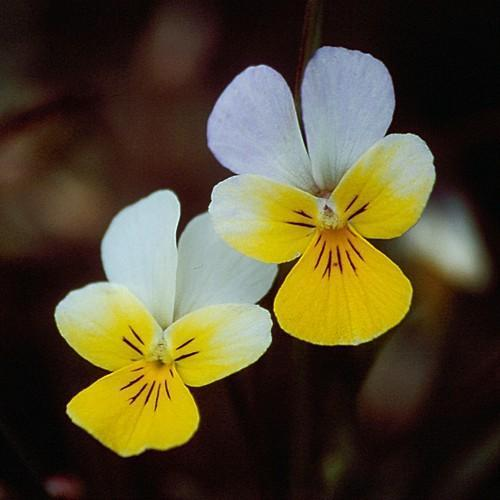
\includegraphics[scale=0.25]{images/original.jpg}
    \caption{Original picture}
    \label{original}
\end{figure}

The script we have implemented would apply the following transformations: 

\begin{figure}[H]
    \begin{subfigure}[t]{0.45\textwidth}
    \centering
  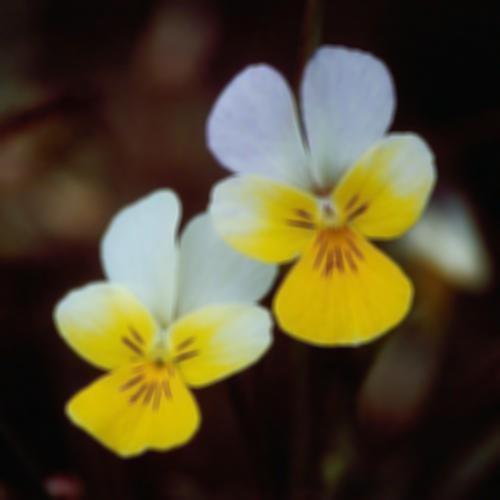
\includegraphics[scale=0.25]{images/blur.jpg}
    \caption{Blur transformation}
    \label{blur}
    \end{subfigure}
    \begin{subfigure}[t]{0.45\textwidth}
    \centering
    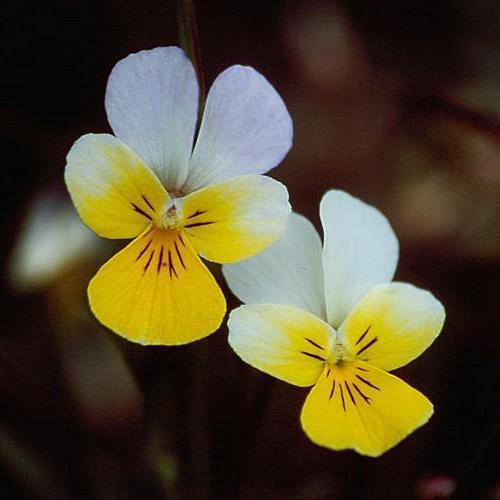
\includegraphics[scale=0.25]{images/horizontal.jpg}
    \caption{Horizontal Flip transformation}
    \label{horizontalflip}
    \end{subfigure}
\end{figure}

\begin{figure}[H]
    \begin{subfigure}[t]{0.45\textwidth}
    \centering
  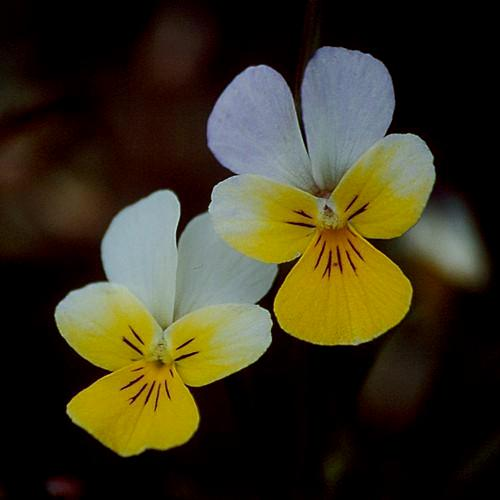
\includegraphics[scale=0.25]{images/brightness.jpg}
    \caption{Brightness and Contrast transformation}
    \label{brightness}
    \end{subfigure}
    \begin{subfigure}[t]{0.45\textwidth}
    \centering
    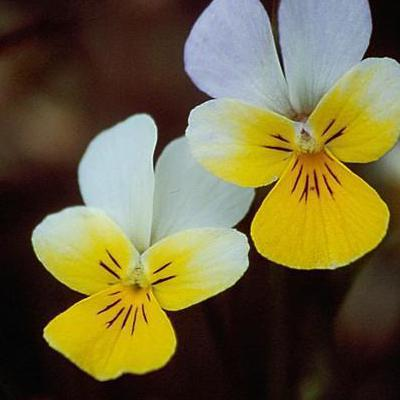
\includegraphics[scale=0.31]{images/scale.jpg}
    \caption{Scale transformation}
    \label{scale}
    \end{subfigure}
    \label{transformations}
    \caption{Data augmentation transformations}
\end{figure}

\section{Results}
\label{sec:results}

The best results have been the KNN Cubic and fitcensemble BAG classifiers, with an accuracy of 80 and 85 respectively. Afterwards, we have modified some parameters of the best classifier in order to obtain even a better accuracy. We have reached a maximum value of XXXX.

\section{List of functions and libraries that have used}
\begin{itemize}
\item \textbf{Bounding Box}: function that finds the relative position of the centroid from the bounding box. It uses the matlab utility \textbf{regionprops} to get the centroid.
\item \textbf{getCompactness}: function that calculates the compactness of a flower. It uses the matlab utility \textbf{regionprops} to get the area. To get the perimeter we have made an erosion and then a substraction. 
\item \textbf{getForma}: function that gets the shape Fourier descriptor. 
\item \textbf{getHog}: function that gets the HOG features. It uses the \textbf{Matlab Computer Vision Toolbox} utility \textbf{extractHOGFeatures}.
\item \textbf{getNumberPetals}: function that gets the number of petals using the skeleton. It uses the matlab utility \textbf{bwmorph} for the skeletonization. 
\item \textbf{getImage}: function that gets us the image and its segmentation.
\item \textbf{segment}: function that segments an image using the active countour method. It uses the matlab utility \textbf{activecontour}.
\item \textbf{image2palette}\cite{image2palette}: Function extracted from Matlab File Exchange. It parses the image into pixels in L*a*b space, and returns the major components clustered by k-means method. The L*a*b color space (defined by the International Commission on Illumination) expresses color as three values: L* for the lightness from black (0) to white (100), a* from green (-) to red (+), and b* from blue (-) to yellow (+). It was designed so that the same amout of numerical change in the values corresponds to the same amount of visually perceived change. We use it to get the 3 main colors of the image and the percentage of pixels in each cluster.

%\item \textbf{histo3d}: function that gets the color information.
\item \textbf{Albumentations library}: for data augmentation issues.
\item \textbf{Google images download library}: to download several pictures of the \textit{zero} class.
\end{itemize}


\newpage
\begin{thebibliography}{100}
\bibitem{image2palette}
	Han. H. (2018). \textit{image2palette: Simple K-means color clustering} [online] Code available at: https://es.mathworks.com/matlabcentral/fileexchange/69538-image2palette-simple-k-means-color-clustering [Accessed 28 April 2019].

\bibitem{Image Segmentation}
\textit{Image Segmentation with MATLAB} [online]. Available at : https://www.mathworks.com/discovery/image-segmentation.html [Accessed 28 May 2019]

\bibitem{Flower dataset}
Nilsback, M-E. and Zisserman, A. (2008) \textit{Automated Flower Classification over a Large Number of Classes} [online] Available at:http://www.robots.ox.ac.uk/~vgg/publications/papers/nilsback08.pdf [Accessed 26 May 2019]


\bibitem{Shape Analysis & Measurement}
M.A. Wirth.(2004) \textit{Shape Analysis \& Measurement} [online] Available at: http://www.cyto.purdue.edu/cdroms/micro2/content/education/wirth10.pdf [Accessed 24 May 2019].

\bibitem{Albumentations}
    Buslaev A.(2018). Based on \textit{Albumentations: fast and flexible image augmentations} [online]. Paper available at:https://arxiv.org/abs/1809.06839. Code available at: https://github.com/albu/albumentations  [Accessed 3 June 2019].


\bibitem{Google images download}
    Vasa H. (2019). \textit{Python Script to download hundreds of images from 'Google Images'.} [online] Code available at: https://github.com/hardikvasa/google-images-download [Accessed 4 June 2019].



%%%%%%%%%%%%%%%%%%%%%%%%%%%%%%%%%%%%%%%%%%%%%%%%%%%%%%%%%%%%%%%%%%%%%%%%%%%%%%%%%%%%%%%
%\bibitem{Analysis of image Thresholding Methods for application to augmented reality enviornments}
%D. Martín Carabias (2012). \textit{Analysis of image Thresholding Methods for application to augmented reality enviornments.} [online] UCM. Available at: https://eprints.ucm.es/16932/1/Tesis\_Master\_Daniel\_Martin\_Carabias.pdf [Accessed 14 Mar. 2019].


%\bibitem{A survey of Thresholding Techniques}
%P. K. Sahoo, S. Soltani, K.C. Wong and Y.C. Chen (1988). \textit{A survey of Thresholding Techniques}. University of Waterloo, Waterloo, Canada  [Accessed 16 Mar. 2019].

%\bibitem{}N. Otsu, \textit{A Threshold Selection Method from Gray-Level Histograms}, in IEEE Transactions on Systems, Man, and Cybernetics, vol. 9, no. 1, pp. 62-66, Jan. 1979.
%[online] Available at http://ieeexplore.ieee.org/stamp/stamp.jsp?tp=\&arnumber=4310076\&is
%number=4310064 [Acessed 17 Mar. 2019].

%\bibitem{}Dr. Andrew Greensted (2010), \textit{Otsu Thresholding}. [online]. Available at http://www.labbookpages.co.uk/software/imgProc/otsuThreshold.html [Accessed 17 Mar. 2019].

%\bibitem{}Senthilkumaran,  N.  \&  Sivapriya,  M.  (2017),  \textit{Riddler's  Thresholding Algorithm  for  DNA  Image  Using  ISODATA  Modified  Algorithm} Journal  of Information Technology, Vol.3, No.2, pp.41-48. [online] Available at: http://www.ijitjournal.org/volume-3/issue-2/IJIT-V3I2P9.pdf [Accessed 17 Mar. 2019].

\end{thebibliography}

\end{document}
